\documentclass[10pt,a4paper]{scrartcl}

\usepackage[backend=biber,style=bwl-FU ,maxcitenames=2,
backend=biber,natbib=true]{biblatex}
\addbibresource{bibliography.bib}

\usepackage[latin1]{inputenc}


\usepackage{quoting}
\quotingsetup{font=small}

\usepackage{caption}
\captionsetup{tableposition=top,figureposition=bottom,font=small}
\usepackage{url}
\usepackage{longtable}


\usepackage{subfigure}

\usepackage{placeins}
\usepackage{stmaryrd}

\usepackage{hyperref}
\usepackage{amsfonts}
\usepackage{amssymb}
\usepackage{graphicx}
\usepackage{listing}
\usepackage{blindtext}
\usepackage{enumitem}
\usepackage{gensymb}
\usepackage{amsbsy}
\usepackage{subfig}
\usepackage{microtype}
\usepackage[english]{babel}
\usepackage[utf8]{inputenx}
\usepackage{xcolor}
\usepackage{amssymb, amsmath}
\usepackage{stmaryrd}
\usepackage{hyperref}
\usepackage{graphicx}
\usepackage{tablefootnote}
\usepackage{footnote}
\makesavenoteenv{tabular}
\makesavenoteenv{table}
\usepackage{cleveref}
\usepackage{lipsum}
\usepackage{curve2e}
\usepackage{booktabs}
\definecolor{gray}{gray}{0.4}
\newcommand{\bs}{\textbackslash}\\


\author{A. Fasano$^1$ \and M. Aguiar$^3$ \and A. Benoit$^1$ \and A. Bideaud$^1$ \and O. Bourrion$^2$ \and M. Calvo$^1$ \and A. Catalano$^2$ \and A. P. de Taoro$^3$ \and G. Garde$^1$ \and A. Gomez$^4$ \and M. F. Gomez Renasco$^3$ \and J. Goupy$^1$ \and C. Hoarau$^2$ \and R. Hoyland$^3$ \and J. F. Mac\'ias-P\'erez$^2$ \and J. Marpaud$^2$ \and A. Monfardini$^1$ \and G. Pisano$^5$ \and N. Ponthieu$^6$ \and J. A. Rubi\~no Mart\'in$^3$ \and D. Tourres$^2$ \and C. Tucker$^5$ \and A. Beelen$^7$ \and G. Bres$^1$ \and M. De Petris$^8$ \and P. de Bernardis$^8$ \and G. Lagache$^7$ \and L. Lamagna$^8$ \and G. Luzzi$^8$ \and M. Marton$^2$ \and S. Masi$^8$ \and R. Rebolo$^3$ \and S. Roudier$^2$}



\title{The new acquisition technique for fast KIDs based spectrometers}

\begin{document}
	
\maketitle

\begin{abstract}{Abstract}
\color{black}

\emph{Context.} Major features demanded for instruments in contemporary cosmology are: high mapping speed to cover large portion of the sky and multi-frequency capability for the component separation. In order to simultaneously satisfy the two conditions you can design large arrays of photo-noise-limited detectors adopting a spectroscopy technique that allows wide instantaneous Field of View, FoV. In this framework we developed KISS, KIDs Interfero-Spectrometer Survey, a spectrometric-imager dedicated to the secondary anisotropies of the Cosmic Microwave Background Radiation, CMBR. In particular the instrument aims to observe the Sunyaev Zel'dovich effect, SZ: an effect due to the interaction between the cluster of galaxies and the CMBR.

\emph{Method.} We exploit a Fourier Transform Spectrometer, FTS. Instead of distribute the pixels to the different frequencies (e.g. on-chip and grating spectroscopy) we developed a double array sensitive to all the interested frequencies. Thank to the FTS we can, then, separate and reconstruct the spectrum. In the ground-based case like KISS, the drawback from such a technique is that we need to be fast to avoid signal contamination from the atmospheric background fluctuations: the single interferometric figure must be acquired with a stable background to properly convert it in a spectrum where the noise does not become indistinguishable from the signal. It is necessary, thus, to use low time-constant detectors and fast FTS technology. KISS adopts, for such target, two arrays of Kinetic Inductance Detector, KID.

\emph{Results.} We developed a new technique to calibrate the KID raw data. We first demonstrate the feasibility of this technique with a simulation. We, thus, study the performance of such technique for the modulation and the tuning, applying it to real on-sky observations. The acquisition technique has been qualified during the first commissioning campaign. It represents a solution for fast multi-frequency acquisition that exploits KIDs based Fourier transform spectrometry.
\end{abstract}

\newpage

\tableofcontents

\newpage

\section{Introduction}
Contemporary cosmology at millimetre wavelengths requires multi-wavelengths study for foregrounds subtraction (e.g. thermal dust, synchrotron, dusty and radio galaxies) and components separation of the various effects for the Cosmic Microwave Background.

In this framework, the necessity to observe at different frequencies makes suitable the exploitation of spectrometers. Among this category a candidate is the FTS. The Fourier Transform  technique applied to spectrometry is a method that exploits the interference of light rather than separate the wavelengths and, compared to competitors (on-chip (\cite{deshima}) and grating (\cite{grating}) spectroscopy), FTS allows larger instantaneous FoV.

Firstly, as in the past for FIRAS (\cite{FIRAS}), the selection of the FTS for the will of developing an instrument fells on a Martin Puplett: an interferometer that measures the difference between the powers of their two input beams (\cite{mpi}). The Martin Puplett Interferometer transposes the observing frequencies paradigm from time to spacial domain and allows to use a calibration source: an ideal choice for precise measurements.

Secondly, the necessity to go fast on data acquisition makes suitable to choose fast detectors like KIDs (for an overview see \cite{kids}). Taking in consideration these premises, using a ``brute-force'' acquisition technique, where you just stock all the information available, would result on a huge data production. In this scenario, it is desirable to adopt a smart solution that minimises the amount of data.

Aiming this optimisation, we want to describe the method developed for KISS.

In sec. \ref{sec:acq} we introduce the method used in past for NIKA2 and it explained the new created for KISS. In the same section it is deeply described the new method and showed a preliminary simulation that allowed the utilisation of the same for the data.

In the sec. \ref{sec:results} we present the first results characterisation of on-sky data.




%\newpage
%\section{The KISS experiment}
%\input{2.kiss/2.tex}

\newpage
\section{The acquisition technique}
\label{sec:acq}

The KID is a superconducting resonator that measures the density variation of the quasi-particles in the lattice, due to photon absorption. It is read-out by a bias line, injecting a tone at its correspondence resonant frequency; at this peculiar frequency, in fact, the coupling between the resonator and the readout line results in an energy absorption, aka band-stop filter. Its time constant is fixed by the recombination time of the quasi-particles from $10 \mu s$ to $100 \mu s$. This represents a major advantage with respect to competitors that are, indeed, a factor $\gtrsim$10 slower.

The $S_{21}$ signal (output/input ratio) related to the KID detector is studied in the complex plane $(I,Q)$, where the resonance shape corresponds to a circle.
The conversion of the $(I,Q)$ signal to absorbed optical power is one of the most difficult challenge using KIDs and it represents a different issue to readout, e.g., thermal detectors (bolometer, TES et cetera).

\subsection{Circular fitting: necessities and constraints}

Smart readout technique is required to properly study the signal and do not encounter huge amount of data. In the past, e.g. for NIKA, an innovative readout technique has been developed (see \cite{Calvo2013} for a detailed discussion). 
The idea, as described in \cite{Catalano2014} , has been to replace the standard fixed excitation (single frequency) tone with a modulated input based on two different frequencies separated by $f_{LO}$: $f_+ = f_0 + \delta f_{LO}/2$ and o$f_- = f_0 - \delta f_{LO}/2$, where $f_0$ is the resonant frequency. This modulation is synchronized to the FPGA sampling of the signal at $\sim$24 Hz. Each raw data point is, thus, composed of the values $(I(t), Q(t))$ and the corresponding differential values:

\begin{equation}
\left( \frac{dI}{df}(t),\frac{dQ}{df}(t) \right) = \left( \frac{I(f_+)-I(f_-)}{\delta f_{LO}}, \frac{Q(f_+)-Q(f_-)}{\delta f_{LO}} \right) \text{ .}
\label{eq:didq}
\end{equation}

\noindent In this way, if a variation $(\Delta I(t), \Delta Q(t))$ occurs between two successive points, it is possible to estimate the corresponding shift in the resonant frequency, $\Delta f_0(t)$, by projecting
$(\Delta I(t), \Delta Q(t))$ along the gradient found, using 
eq. \ref{eq:didq}:

\begin{equation}
\Delta \hat{f}_0 (t) = \frac{(\Delta I(t), \Delta Q(t))\cdot (dI/df(t),dQ/df(t)  ) }{ ( dI/df(t), dQ/df(t) )^2 }\cdot\delta f_{LO} \text{ ,}
\end{equation}

\noindent we refer to $\Delta \hat{f}_0 (t)$ as $RFdIdQ$.

The constraints over the data acquisition are slightly more demanding in KISS: two consecutive interferograms are acquired at 5 Hz, to overcome the 1/f atmospheric noise at $\sim$1 Hz, and the data rate is quite higher, 3.816 kHz, in order to obtain the aimed spectral resolution of few GHz. In this condition it is not possible to modulate the signal each single point, because the FPGA does not reach the necessary rate and you would, eventually, manage a factor 2 on data weight.

\subsection{Modulation: the algorithm to obtain physical data}
\label{sebsec:alg}

The idea for KISS is to obtain the physical conversion through a modulation but, in this case, the mechanism is different. First of all the spectral information is in data block containing the forward and backward interferograms: a moving mirror oscillates generating the optical path difference that results in the interferogram figures, one per oscillation direction. That is the main difference with NIKA2: KISS is a interferometer. This repetitive block of points is composed as following: in the first part it is injected a frequency $f_+ = f_0 + \Delta f_{LO}/2$, in the second a frequency $f_- = f_0 - \Delta f_{LO}/2$ and for the rest the frequency of resonance $f_0$, as we can see in fig. \ref{fig:mod}.

\begin{figure}[htf]
	\centering
	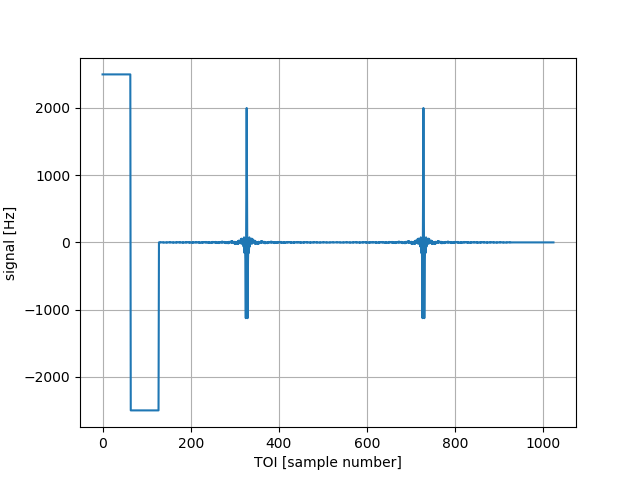
\includegraphics[width=.5\textwidth]{3.acqui/block_data.png}
	\caption{Data block simulation of KISS: signal [Hz] vs Time Ordered Information, TOI, [sample number]. There are a total of 1024 points: the first 128 dedicated to the modulation and the rest to incoming signal. We simulate the forward and backward interferograms with a typical amplitude of 2 kHz and the shape of the black body at 3 K and 30 K.}
	\label{fig:mod}
\end{figure}

\noindent The choice over the total number of points for one block, including the ones assigned to the modulation, takes into account few major constraints: the spectral resolution aimed to $\sim$1 GHz requires a displacement of the mirror of 10 cm; the cut-off of the KID time constant $\sim$100 $\mu$s, that limits the single datum acquisition rate; the fast (5 Hz) scan requirement to avoid the 1/f atmospheric noise. The result consists on a total period of 1024 points, where each point is acquired at 3.816 kHz, dedicating the first 128 to the modulation. In this way we have $\sim$400 points each interferogram, obtaining $\sim$100 points on the interested spectrum frequencies.

\noindent We can extrapolate the calibration factor $C$ [Hz/rad] through a circular fit on the modulation points $(x1,y1)$ and $(x2,y2)$, referring to fig. \ref{fig:IQ_modulation}. We obtain, in this way, the coordinates of the circle centre $(I_c,Q_c)$. We can calculate, thus, the $r_1$ and $r_2$ angles as following:

\begin{equation}
\begin{align}
r_1 &= \arctan\left( \frac{I_c-x_1}{Q_c - y_1}  \right) &\text{ ,}\\
r_2 &= \arctan\left( \frac{I_c-x_2}{Q_c - y_2}  \right) &\text{ .}
\end{align}
\end{equation}

\noindent The modulation factor $C$ is obtained as following:

\begin{equation}
\begin{align}
\Delta \phi &= r_2-r_1 &\text{ ,}\\
C&=\Delta\phi/\Delta f &\text{ ;}
\end{align}
\end{equation}

\noindent where $\Delta f$ is the modulation in hertz set by the injecting tone.

\begin{figure}[htf]
	\centering
	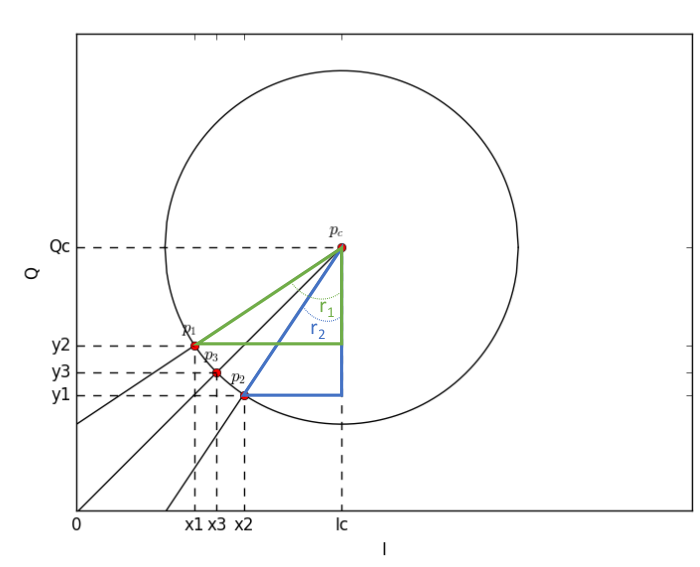
\includegraphics[width=0.5\textwidth]{3.acqui/circle.png}
	\caption{Resonance circle in the $(I,Q)$ plane. $p_1$ and $p_2$ are the modulation points, $p_3$ is the measurement point and $p_c$ is the circle centre. }
	\label{fig:IQ_modulation}
\end{figure}

\noindent Operatively, $C$ converts the observing phase, $\phi=\arctan\left( \frac{I}{Q} \right)$, to hertz data, the physical quantity (as seen in \cite{Swenson}) that can be used to obtain the incoming power in watts.


\subsection{Simulation}

In order to understand if and under which conditions this method is valuable work we use the characterising values $f_0$, resonance frequency, $Q_i$, internal quality factor, and $Q_c$, coupling quality factor, obtained in laboratory from the actual KISS arrays tests to fit the skewed Lorentzian profile \cite{Gao}:

\begin{equation}
	\left|S_{21}(f)\right|= \alpha+\beta(f-f_0)+\frac{\gamma+\delta(f-f_0)}{1+4Q_{tot}^2\cfrac{(f-f_0)^2}{f_0^2}} \text{ ,}
	\label{eq:s21_amp}
\end{equation}

\noindent where $\alpha$, $\beta$, $\gamma$ and $\delta$ are factors that do not influence the parameters on study. With eq. \ref{eq:s21_amp} we can extrapolate $Qi$ (\cite{Gao}):

\begin{equation}
Q_i =\frac{Q_{tot}}{min(\left|S_{21}(f)\right|)}
\end{equation}

\noindent In this way we simulate the KIDs used for KISS qualifying them for the modulation technique. In fig. \ref{fig:fit_amp} and \ref{fig:hist} we have the typical KISS electrical measurements in laboratory.

\begin{figure}[htf]
	\centering
	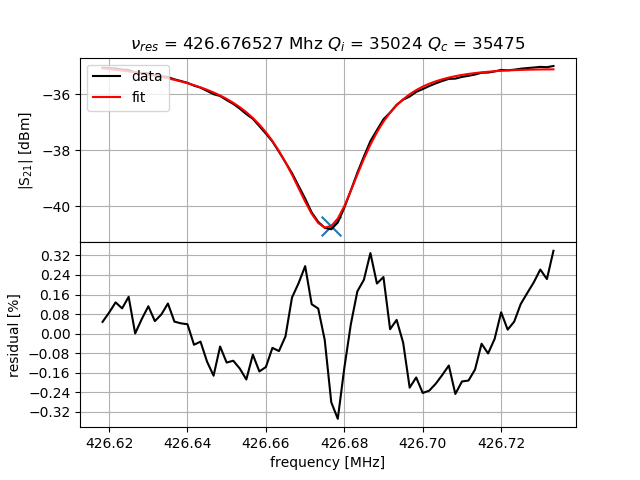
\includegraphics[width=.5\textwidth]{3.acqui/resonance_fit.png}
	\caption{Up: single pixel bias signal data (in black) fitted (in red) by \ref{eq:s21_amp}. Bottom: percentile residual between fit and data.  Typical fit using eq. \ref{eq:s21_amp} on a KISS pixel in laboratory. In this case we notice that the quality factors are coupled (aka similar), this condition maximised the responsivity (\cite{Gao}).}
	\label{fig:fit_amp}
\end{figure}

\begin{figure}[htf]
	\centering
	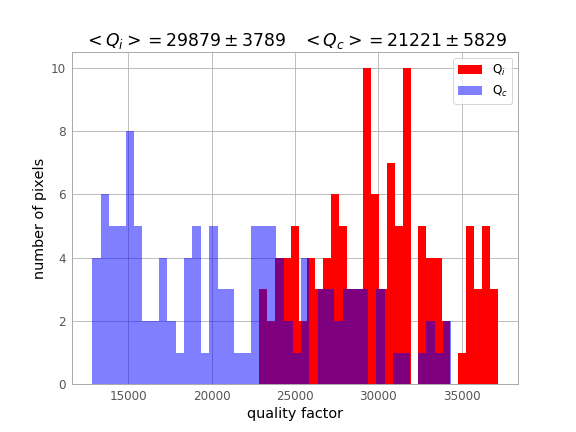
\includegraphics[width=.5\textwidth]{3.acqui/Q_hist.png}
	\caption{Quality factors histograms measured on the KISS array. In red the internal quality factor with a background of 50 K, that simulates the sky and in blue the coupling quality factor.}
	\label{fig:hist}
\end{figure}

\noindent At this point we can proceed simulating the resonator in the complex plane with the equation (\cite{Gao}):
\begin{equation}
S_{21}(f)=ae^{-2\pi j f \tau} \left[ 1-\frac{\frac{Q_{tot}}{Q_c}e^{j\phi_0}}{1+2jQ_{tot}\left(\frac{f-f_0}{f_0}\right)}\right] \text{ ,}
\label{eq:s21_IQ}
\end{equation}

\noindent using the values in tab. \ref{tab:s21_values}, where , $Q_{tot}\doteq\left( 1/Q_i + 1/Q_c \right)^{-1}$ and $\mathfrak{R}$ is the responsivity measured during laboratory test; $\tau$ is the retard introduced by the cables and $\phi_0$ is a phase, they are not taken into account for this study.

\begin{table}[htf]
	\footnotesize
	\centering
	\caption{Input values from laboratory characterisation taken from fig. \ref{fig:hist} for the resonator simulation.}
	\begin{tabular}{cc}
		\toprule
		\textbf{parameter} & \textbf{value} \\
		\toprule
		$\tau$ & 1 \\ 
		\midrule 
		$\phi_0$ & 0 \\
		\midrule
		$f_0$ & 500 MHz \\  
		\midrule 
		$Q_i$ & 30'000 @ 50 K \\ 
		\midrule 
		$Q_c$ & 21'000 \\ 
		\midrule 
		$\mathfrak{R}$  & 1.5 kHz/K \\ 
		\bottomrule
	\end{tabular}
\label{tab:s21_values}
\end{table}

\noindent We, thus, obtain the $\left|S_{21}(\nu)\right|$ shape as shown in fig. \ref{fig:s21_simu}.

\begin{figure}[htf]
	\centering
	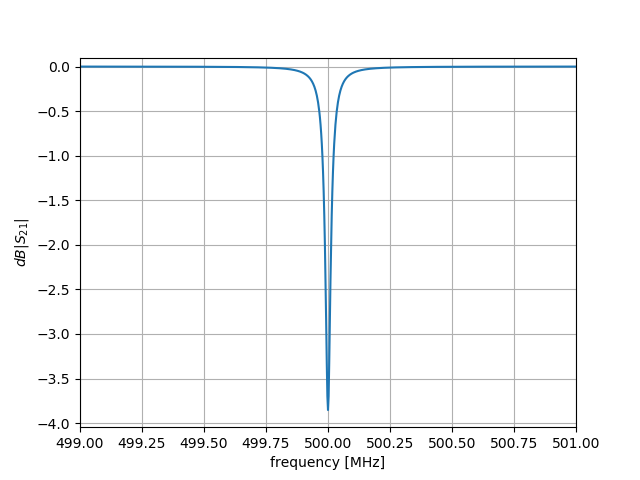
\includegraphics[width=.5\textwidth]{3.acqui/resonance.png}
	\caption{$\left|S_{21} \right|$ signal [dB] (simulated using eq. \ref{eq:s21_IQ} with input values of tab. \ref{tab:s21_values}) vs frequency [MHz]. It represents the typical KISS pixel. }
	\label{fig:s21_simu}
\end{figure}

First of all, starting from these simulated data we generate a data block with assigned modulation factor and interferogram amplitude, $A$, in hertz. The second step is to use these hertz data with eq. \ref{eq:s21_IQ} obtaining the values in quadrature $(I,Q)$. From them we compute the phase $\phi=\arctan\left(\frac{I}{Q}\right)$. Finally we come back to hertz signal through the calibration algorithm described in sec. \ref{sebsec:alg}. We, thus, compare the modulation factor and interferogram amplitude in input, $C_{in}$ and $A_{in}$ and output, $C_{out}$ and $A_{out}$, of this algorithm. This verification is necessary for understanding the reliability of the calibration method. In fig. \ref{fig:cal_bck} we report the change on the calibration factor as a function of background, at fixed modulation factor and interferogram amplitude.

\begin{figure}[htf]
	\centering
	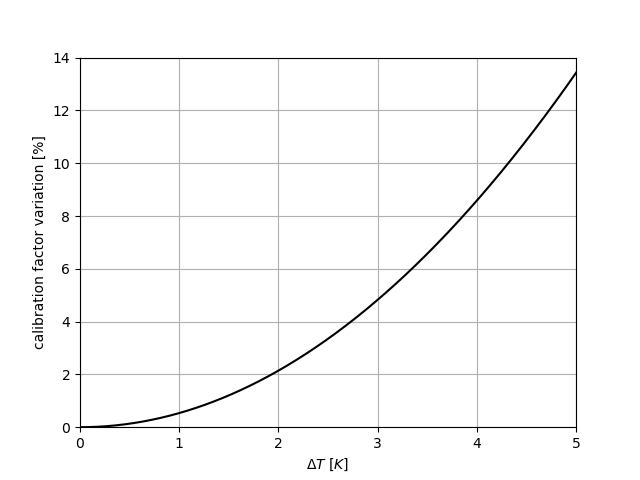
\includegraphics[width=.5\textwidth]{3.acqui/calibration_factor_variation.png}
	\caption{Calibration factor percentile variation, $\frac{C_{out}-C_{in}}{C_{in}}$, [Hz/rad] vs background variation [K]. The modulation factor, $\Delta f$, is fixed at at 2.5 kHz. The calibration factor, $C_{out}$, is independent to different $A_{in}$.}
	\label{fig:cal_bck}
\end{figure}

\noindent In fig. \ref{fig:amp_bck} we show the variation on the estimation of the interferogram amplitude, at fixed modulation factor: we see how this estimation is degradated at large background variations.

\begin{figure}[htf]
	\centering
	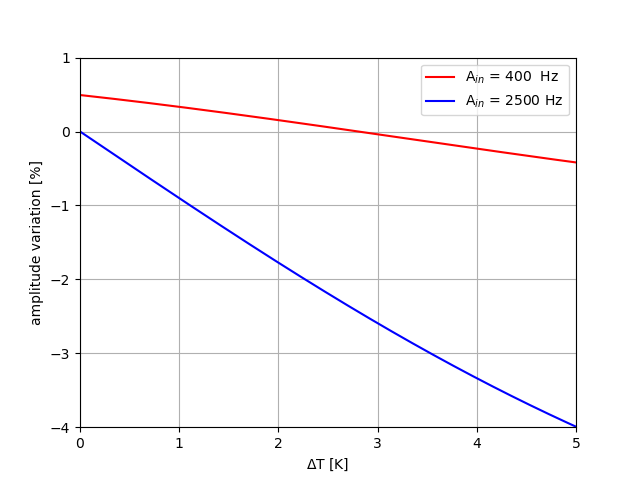
\includegraphics[width=.5\textwidth]{3.acqui/amplitude_variation.png}
	\caption{Interferogram amplitude percentile variation, $\frac{(A_{out}-A_{in})}{A_{in}}$, estimation vs background [K]. The modulation factor $\Delta f$ is fixed at 2.5 kHz. We can see how the higher value of the amplitude degrades the method}
	\label{fig:amp_bck}
\end{figure}

\noindent In fig. \ref{fig:amp_mod} we show the last result of the simulation: every curve is at different, fixed interferogram amplitude and the figure represents the variation on the amplitude estimation in function of different calibration factors. As expected, we want to be as close as possible between the calibration factor and the amplitude variation. Other choices could compromise the amplitude estimation of maximum $\sim$1\% that is, still, an acceptable compromise.

\begin{figure}[htf]
	\centering
	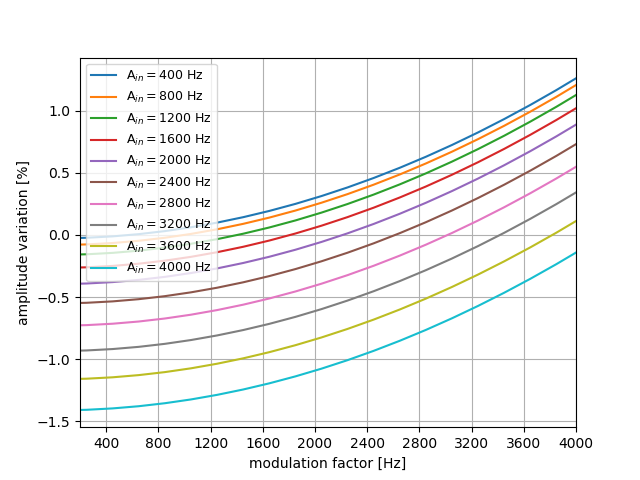
\includegraphics[width=.5\textwidth]{3.acqui/several_modulations.png}
		\caption{Every curve is at different interferogram amplitude $A_{in}$. Interferogram amplitude percentile variation, $\frac{A_{out}-A_{in}}{A_{in}}$, vs modulation factor $\Delta f$.  The background is fixed at zero. We can see how the error on the estimation converges to 0 when $\Delta f$ approaches $A_{in}$. }
	\label{fig:amp_mod}
\end{figure}

\subsection{Tuning procedure}
\label{sec:tuning}

The new modulation technique for KISS, described and simulated in the previous sections is the major improvement on the data calibration and production. On the other side, to optimise the working point of the KID it is necessary to retune: while you observe, the atmospheric fluctuations modify the resonance. What is done at the end of each observation, in the standard perspective, is a full frequency sweep to retune the resonance frequency: this represents a time-demanding procedure. By the way we can, similarly to NIKA2, adopt a strategy that permits to save $\sim$75\% of time in the pre-observation phase of retuning, this strategy is detailed explained in (\cite{2014SPIE.9153E..02C}). At first, you measure the angle $\Phi$ between the vectors $(I,Q)$ and $(dI/df_{LO},dQ/df_{LO})$ referring to eq. \ref{eq:didq} and you define, for convenience, a new angle $\theta\doteq \pi/2-\Phi$ that changes smoothly around $[-\pi,\pi]$. Secondly, the excitation tone is fixed at $\theta=0$ and you estimate the $\theta(f)$ slope $\Delta\theta/\Delta f'$. Then, you vary the tone frequency $f^i$ monitoring $\theta^i$. And finally, you can evaluate the new resonance frequency:

\begin{equation}
f^i_0 \simeq f^i - \frac{\theta^i(t)}{\Delta\theta/\Delta f'} \text{ .}
\end{equation}

The procedure described in this section is used for KISS. It represents a resilient tool that can be adopt on KIDs-based experiments: even for large background fluctuations, you can iterate the algorithm to converge.




\newpage
\section{Results}
\label{sec:results}

\subsection{Algorithm on real data}

In this section we show the first results obtained from the first part of the commissioning campaign of the instrument, installed at the QUIJOTE telescope in Tenerife. We can see in fig. \ref{fig:circle} the circular fit performed on real data as described in fig. \ref{fig:IQ_modulation}: the two external are the modulation points and the central distribution represents the variation of the signal during the observations.


\begin{figure}[htf]
	\centering
	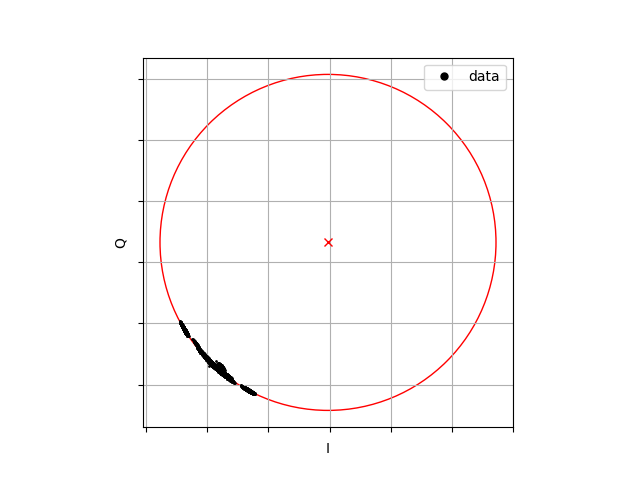
\includegraphics[width=.5\textwidth]{4.results/circular_fit.png}
	\caption{Observation in $(I,Q)$ plan: in black dots the data and in red shape the circular fit. We can see the two modulation (external) points and the central distribution due to the signal changing during the observation [scan 283, pixel KA001]}
	\label{fig:circle}
\end{figure}

\noindent Operatively, the circular fit showed in fig. \ref{fig:circle} is used in two different ways and represents a crucial tool during the observations, as well as for the data analysis. Firstly, during the observation, it gives an important visual feedback to understand if the tuning (as seen in sec. \ref{sec:tuning} ) is correctly working. Secondly, it is one of the first step in the conversion algorithm for the physical data analysis, as already described in sec. \ref{sebsec:alg}.

The first result, that we can compare with the simulation, is reported in fig. \ref{fig:calfact}: it is the calibration factor estimated as a function of TOI during a sky observation. Every point corresponds to a data block (sampled at 5 Hz).

\begin{figure}[htf]
	\centering
	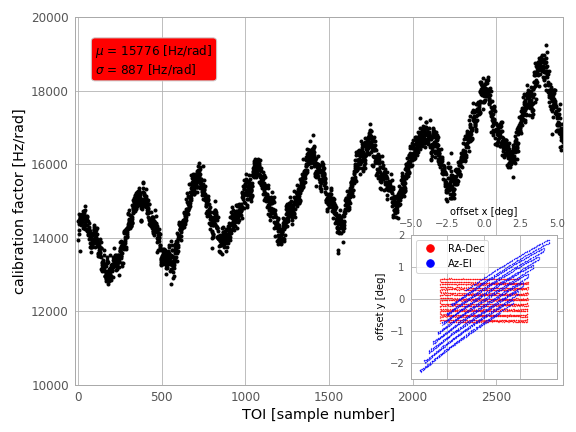
\includegraphics[width=.7\textwidth]{4.results/calfact.png}
	\caption{Calibration factor as a function of Time Ordered Information, TOI, during an observation. The gaussian fit reported in the red top-left box is evaluated from the data that have beed before median filtered. We can notice the derive of the calibration factor due to the Right-Ascension Declination (RA-Dec) observation: the telescope increases the elevation following the source. In the bottom-right the offset maps of the sky-coordinates in RA-Dec and Azimuth-Elevation.}
	\label{fig:calfact}
\end{figure}


Here we assume the background fluctuation, as seen in fig. \ref{fig:cal_bck}, as unique source of incertitude for the calibration factor estimation: we consider the noise contamination negligible, let's first demonstrate this assumption. We take the median of the $ASD$, $\tilde{ASD}$, as its equivalent white noise level: it is (taking margins) $\sim$1 $Hz/\sqrt{Hz}$.

\noindent  We can, then, use the definition of the standard deviation of the TOI noise signal:

\begin{equation}
\sigma \doteq \int_{0}^{\Delta f} [ASD(f)]^2\cdot df \text{ ,}
\label{eq:sigma}
\end{equation}

\noindent where $ASD(f)$ is the $ASD$ as a function of frequency $f\in[0,\Delta f]$, $\Delta f$ is the bandwidth equal to half of the sampling frequency (for the Nyquist theorem) and $df\doteq\Delta f/N$, with $N$ is the number of the points.

\noindent Approximating $ASD$ in eq. \ref{eq:sigma} as a pure white noise, $\tilde{ASD}$, we obtain:

\begin{equation}
\sigma\simeq \sqrt{ \tilde{ASD}^2 \cdot \Delta f } \text{ ,}
\end{equation}

\noindent Finally, in tab. \ref{tab:sigma_sig}, we can see the typical fluctuations of the signal as a function of sampling rate: compared to the background variation (equivalent of $\sim 1$ kHz) simulation in fig. \ref{fig:calfact} it represents, Q.E.D., a very small components.

\begin{table}[htf]
	\footnotesize
	\centering
	\caption{From eq. \ref{eq:sigma} typical rounded-up 1-$\sigma$ noise signal.}
	\begin{tabular}{ccc}
		\toprule
		\textbf{mode} & \textbf{bandwidth [Hz]} & \textbf{$\sigma$ [Hz]} \\
		\toprule
		single point & 1908 & $\sim$50 \\ 
		\midrule 
		block data & 2 & $\sim$2 \\ 
		\bottomrule
	\end{tabular}
	\label{tab:sigma_sig}
\end{table}

Starting from this paradigm we can, thus, compare the results of the simulation with on sky observations. In the first scenario there is a $\lesssim 3\%$ variation of the calibration factor each kelvin background fluctuation, as shown in fig. \ref{fig:cal_bck}. What we notice on sky (fig. \ref{fig:calfact}) is a fluctuation $\sigma/\mu\sim6\%$, where $\sigma$ is the standard deviation and $\mu$ the mean value of the calibration factor. We can conclude that during a typical $\sim$4$\textdegree$ scan we have temperature fluctuation of the sky $\lesssim 2$ K.


\subsection{Algorithm validation}
The purpose of this study is to qualify the new technique developed for KISS: modulation and auto-tuning.

\color{red}
To insert validation of calibration.
\color{black}

Secondly, what we need to state that the acquisition/data-reduction system is qualified for the instrument is to observe if the auto-tuning (sec. \ref{sec:tuning}) works. For this purpose, we take three consecutive maps at different elevations: we plot the $(I,Q)$ data of the first subscan for each map observing the behaviour of the acquisition referring the circular fit to the first tuning (corresponding to the first map). The result is shown in fig. \ref{fig:autotuning}.

\begin{figure}[htf]
	\centering
	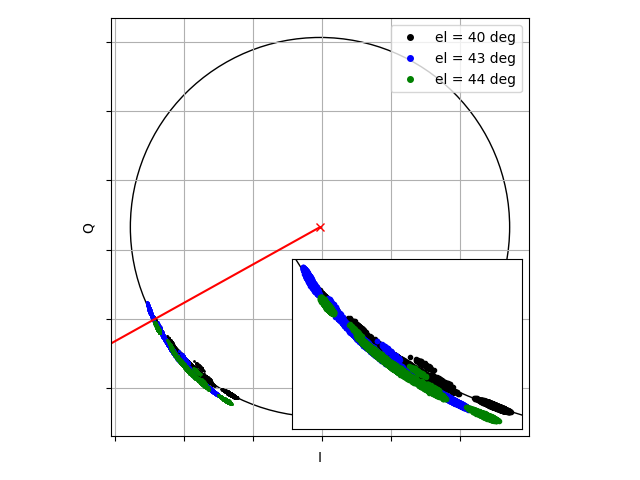
\includegraphics[width=.5\textwidth]{4.results/autotuning.png}
	\caption{$(I,Q)$ signal of the first subscan for three consecutive maps, i.e., different elevations. The red straight line is the intercept between the origin and the circle centre.}
	\label{fig:autotuning}
\end{figure}

\noindent We can see how the data are disposed on the same region close to the ones of the first circle, they are around the intercept between the centre of the circle the origin: it means that they are around the minimum of the resonance, i.e., to the frequency of resonance. The data are not perfectly centred because of the intrinsic incertitude on the binning of the injected tone. The radial shift is due to the background change: different elevations correspond to a different air mass, $\sim 1/\cos(el)$. The tuning technique performed between each map recover the resonance  tone, adapting it to the background change.

\newpage
\section{Conclusions and Perspectives}
The purpose of this paper is to demonstrate and explain the new acquisition technique for KISS. As previously mentioned, this algorithm is naturally implementable for all those instruments that will aim to exploit KID-based interferometers: a worthwhile solution for the contemporary and future multi-wavelength cosmology. Although KISS represents a standalone instrument to make science, it opens future perspectives for larger arrays experiments. Specifically for these cases, in fact, our new algorithm will minimise the data production and contain the inflation on the electronics specifications.

%\section*{Appendices}
%\subsection*{A. SZ effect}
%\input{A.SZ/sz.tex}

\newpage
\nocite{}
\printbibliography

\end{document}

